% CONTEXT
\chapter{Contexte et cahier des charges}


% PERSONAL PERSPECTIVES
\section{Perspectives personnelles}
Cette expérience professionnelle s'inscrit dans le cadre de mon stage de fin d'année en Licence 3 Sciences pour l'Ingénieur, parcours Informatique, à la Faculté des Sciences et Techniques de l'Université de Corse. J'ai été accueilli par l'entreprise DEPT, au sein de son département en Irlande.

J'ai choisi ce stage afin d'approfondir mes connaissances dans le domaine du web, de découvrir le monde de l'entreprise et de comprendre les méthodes de travail dans un contexte international. Cette opportunité de travailler dans une entreprise située hors de France m'a permis de découvrir de nouvelles pratiques professionnelles. Je suis très honoré de pouvoir apporter, à mon modeste niveau, une contribution à une entreprise de portée mondiale.


% PRESENTATION UNIV & PROJECT
\section{Présentation de DEPT et ses projets}
\subsection{Présentation}
DEPT a été créer en 2005 à Amsterdam au Pays-Bas c'est une entreprise innovante dans les domaines de la technologie et du marketing, aidant ses clients à rester à la pointe. En tant qu'agence numérique complète, DEPT réunit plus de 4 000 experts répartis sur plus de 30 sites à travers cinq continents. Travaillant avec des clients prestigieux tels qu'Adidas, Patagonia, Google Workspace, et bien d'autres, DEPT combine créativité et technologie pour offrir des expériences numériques globales, optimisant chaque étape du parcours client. De plus, l'entreprise conçoit, développe et intègre des solutions logicielles et matérielles pour les principales sociétés SaaS et traditionnelles.

\subsection{Projets de l'entreprise}
Du commerce électronique et des technologies émergentes aux expériences client et à l'architecture \footnote{Le cloud est un ensemble de serveurs distants utilisés pour stocker, gérer et traiter des données via Internet.}cloud, Dept imaginne et met en œuvre des solutions techniques d'avenir qui établissent de nouvelles normes pour les entreprises numériques.
\\ \\
DEPT a réalisé de nombreux projets en voici des exemples.


\subsubsection{Arizona State University}

DEPT collabore avec l'Arizona State University (ASU) pour rendre l'éducation plus accessible et équitable à travers le développement de plateformes éducatives adaptées aux besoins spécifiques des apprenants du monde entier. Depuis plus de six ans, DEPT et ASU ont créé diverses solutions EdTech, notamment:

\begin{itemize}
    \item \textbf{Baobab}: Application pour le réseautage et le mentorat des jeunes leaders africains.
    \item \textbf{me3®}: Outil interactif de planification de carrière basé sur un modèle \footnote{SaaS signifie "logiciel en tant que service". C'est un modèle où les logiciels sont hébergés sur le cloud et accessibles via Internet.}SaaS.
    \item \textbf{Young Thinkers}: Programme en ligne de préparation à l’université et à la carrière pour les jeunes émiratis et arabes.
    \item \textbf{Intelligent Tutor}: Tuteur intelligent pour l'apprentissage autonome en mathématiques.
\end{itemize}

En utilisant une approche centrée sur l'utilisateur, DEPT garantit que chaque solution est adaptée aux contraintes techniques et culturelles des apprenants, contribuant ainsi à démocratiser l'éducation et à atteindre plus d'un million d'utilisateurs à travers le monde.

\subsubsection{Fingerspelling}

HELLO MONDAY/DEPT® et l'American Society for Deaf Children ont créé \textbf{Fingerspelling.xyz}, une application web utilisant l'apprentissage automatique pour enseigner l'alphabet de la langue des signes américaine (ASL).

Fingerspelling.xyz utilise \textit{MediaPipe Hands} pour suivre les mouvements des mains via une webcam. Un modèle 3D montre comment positionner les mains pour chaque lettre, avec des retours en temps réel.

L'application a enregistré des millions de signes corrects et est utilisée par l'American Society for Deaf Children. Récompenses :
\begin{itemize}
    \item \textbf{Webby Awards 2023}: trois People's Voice Awards. 
    \item \textbf{Webby Awards 2022}: deux Webby Awards et trois People's Voice Awards.
    \item \textbf{Eurobest Awards}: Prix de l'innovation, Or en design.
    \item \textbf{Awwwards}: Site du jour.
    \item \textbf{FWA}: Site du jour et du mois.
    \item \textbf{Cannes Lions}: Or et Argent en design.
    \item \textbf{New York Design Awards 2021}: Argent.
    \item \textbf{Anthem Awards}: Or en Éducation.
\end{itemize}

Fingerspelling.xyz améliore la communication et l'inclusion pour la communauté des Sourds.

\subsection{Participation à l'entreprise}

Dept à de nombreux clients dans l'ecommerce et cherche à concevoir des solutions pour automatiser, éviter de la répétition de taches et améliorer la cohésion entre les différents professionnelles dans le processus de développement et de création
\\ \\
L’équipe qui s’occupe du développement de cet solution est composé de trois personnes : 
\begin{itemize}
    \item M. Derek Brady est le directeur créatif et associé chez DEPT, il s'occupe sur la vision à long terme de l'entreprise, il supervise et à dirige la création et le développement des aspects visuels et créatifs des projets.
    \item M. Marc Raffalli est développeur \footnote{Le front-end est la partie d'une application ou d'un site web avec laquelle les utilisateurs interagissent directement. Cela inclut l'interface utilisateur, le design et les fonctionnalités visibles.}front-end senior, il s'occupe de l'aspects techniques des projets, il s'est occupé de guider et de m'encadrer tout au long du stage
    \item Enfin, Moi-même, stagiaire ayant pour but de créer la solution pour optimier le processus de création avec l'UI et l'UX dynamique.
\end{itemize}

\section{Cahier des charges}
Le but de ce stage est de créer une solution pour automatiser pour la création d'UI et UX dynamique avec \footnote{JavaScript est un langage de programmation de haut niveau principalement utilisé pour créer des fonctionnalités interactives sur les sites web.}Javascript, \footnote{React est une bibliothèque JavaScript open-source utilisée pour construire des interfaces utilisateur interactives et réactives pour les applications web et mobiles.}React et \footnote{Next.js est un framework JavaScript basé sur React, utilisé pour créer des applications web rapides et évolutives.}Next.js pour les futurs clients de l'entreprise, en utilisant des technologies modernes et en respectant les standards de l'entreprise. 
\\ \\
Cette solution doit permettre de gagner du temps, d'éviter les erreurs et de faciliter la communication entre les différents professionnels.

Il m'a été demandé de tester plusieurs outils et services pour voir s'ils peuvent répondre aux problématiques.
Ensuite, il m'a été demandé d'étudier les différentes possiblité d'interactions entre les outils. 

Puis, de créer un prototype de la solution en utilisant Javascript \ref{doc:javascript} avec React \ref{doc:react} et Next.js \ref{doc:nextjs} connecté a un Headless CMS.

Enfin, de tester la solution, de identifié les forces et les faiblesses pour présenter la solution à l'équipe.

% Gestion du temps
\section{Gestion du temps}

Pendant mon stage, j'ai accordé une grande importance à une gestion efficace du temps, afin de maximiser ma productivité et de mener à bien les différentes tâches qui m'ont été confiées. Voici une vue d'ensemble de ma gestion du temps (figure \ref{fig:Diagramme circulaire - Gestion du temps}), basée sur les pourcentages suivants :

\begin{itemize}
\item \textbf{Programmation} : J'ai consacré environ 30\% de mon temps à la programmation. Cela inclut la création le développement en React et Next.js pour créer le prototype de la solution avec la connexion avec le Headless CMS et la mise en place du motif de conception.

\item \textbf{Test des outils} : Environ 25\% de mon temps a été dédié aux tests des outils. J'ai testé les outils Relume, Webflow et Devlink pour voir s'ils répondaient aux besoins du projet et pour identifier les avantages et les inconvénients de chacun.

\item \textbf{Recherche et apprentissage} : Environ 20\% de mon temps a été consacré à la recherche et à l'apprentissage de nouvelles technologies et des nouveaux outils. J'ai appris à utiliser des outils tels que Webflow, Relume et ContentFul pour le headless CMS, et j'ai approfondi mes connaissances en Next.js 14 qui a apporté des changements et nouvelles fonctionnalités.
\item \textbf{Collaboration} : J'ai consacré environ 15\% de mon temps à la collaboration avec l'équipe autour du projet. Cela comprenait des réunions, des discussions et des échanges d'idées pour garantir que le projet prenne la bonne direction, la prise en compte des éventuelles suggestions et la validation de l'avancée de projet.

\item \textbf{Analyse et proposition}: Environ 10\% de mon temps a été consacré à l'analyse des spécifications ; à la proposition de solutions adaptées aux besoins du projet et du cahier des charges. Cette phase m'a permis de comprendre en détail les exigences et d'identifier les meilleures approches pour les satisfaire.
\end{itemize}
\begin{figure}[ht] 
    \centering
    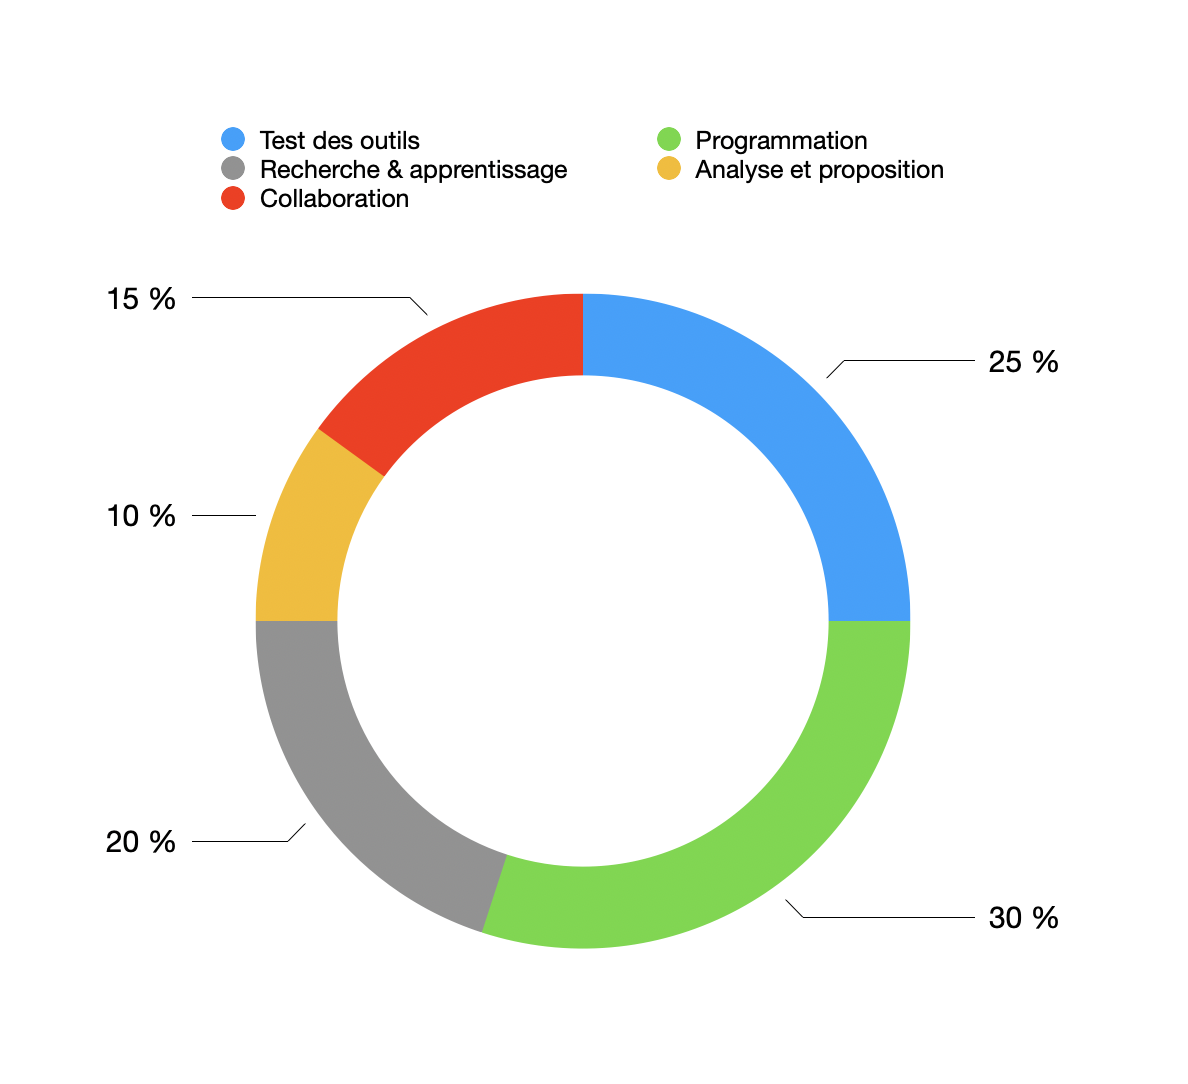
\includegraphics[width=0.7\textwidth]{Includes/Images/gestionTemps.png}
    \caption{Diagramme circulaire - Gestion du temps}
    \label{fig:Diagramme circulaire - Gestion du temps}
\end{figure} 
De ce fait, cette gestion du temps équilibrée m'a permis de mener à bien mes tâches et d'atteindre les objectifs fixés dans les délais impartis. Cette répartition réfléchie du temps m'a permis de rester organisé, de faire face aux défis et d'obtenir des résultats positifs tout au long de mon stage.

\subsection*{Communication et gestion de projets}

Pendant les quatres mois de mon stage, nous avons mis en place une solide gestion de projet, qui nous a permis de progresser de manière efficace et de répondre aux attentes fixées. Dès le début, j’ai reçu le cahier des charges détaillant les objectifs et les exigences du projet. Cela m’a donné une vision claire de ce qui était attendu et j’ai pu commencer à développer en conséquence.

Pour assurer un suivi régulier et des retours constructifs, j’ai adopté une approche itérative dans mon travail. À chaque petite étape ou module que je complétais, je les soumettais à M. Marc Raffalli, mon mentor et developpeur front-end senior. Il examinait attentivement mon travail et me fournissait des retours précieux. J’ai pris en compte ces commentaires et suggestions, ce qui m’a permis d’améliorer continuellement mes réalisations avant de passer à l’étape suivante.
\\ \\
Cette méthodologie agile a permis une flexibilité accrue, une adaptation en temps réel aux changements et une amélioration constante tout au long du processus de développement.
